% Copyright 2004 by Till Tantau <tantau@users.sourceforge.net>.
%
% In principle, this file can be redistributed and/or modified under
% the terms of the GNU Public License, version 2.
%
% However, this file is supposed to be a template to be modified
% for your own needs. For this reason, if you use this file as a
% template and not specifically distribute it as part of a another
% package/program, I grant the extra permission to freely copy and
% modify this file as you see fit and even to delete this copyright
% notice. 

\documentclass{beamer}
\usepackage{graphicx}
\usepackage{amssymb}
\usepackage{amsmath}
\usepackage{amsthm}
\graphicspath{{Images/}}
% Replace the \documentclass declaration above
% with the following two lines to typeset your 
% lecture notes as a handout:
%\documentclass{article}
%\usepackage{beamerarticle}


% There are many different themes available for Beamer. A comprehensive
% list with examples is given here:
% http://deic.uab.es/~iblanes/beamer_gallery/index_by_theme.html
% You can uncomment the themes below if you would like to use a different
% one:
%\usetheme{AnnArbor}
%\usetheme{Antibes}
%\usetheme{Bergen}
%\usetheme{Berkeley}
%\usetheme{Berlin}
%\usetheme{Boadilla}
%\usetheme{boxes}
%\usetheme{CambridgeUS}
%\usetheme{Copenhagen}
%\usetheme{Darmstadt}
%\usetheme{default}
%\usetheme{Frankfurt}
\usetheme{Goettingen}
%\usetheme{Hannover}
%\usetheme{Ilmenau}
%\usetheme{JuanLesPins}
%\usetheme{Luebeck}
%\usetheme{Madrid}
%\usetheme{Malmoe}
%\usetheme{Marburg}
%\usetheme{Montpellier}
%\usetheme{PaloAlto}
%\usetheme{Pittsburgh}
%\usetheme{Rochester}
%\usetheme{Singapore}
%\usetheme{Szeged}
%\usetheme{Warsaw}

\title{On the Birkhoff Conjecture for Convex Billiards}

\author{Han Yong Wunrow\inst{1}}
% - Give the names in the same order as the appear in the paper.
% - Use the \inst{?} command only if the authors have different
%   affiliation.

\institute[Universities of Somewhere and Elsewhere] % (optional, but mostly needed)
{
  \inst{1}%
  Undergraduate Department of Mathematics \\
  University of Minnesota - Twin Cities
}
% - Use the \inst command only if there are several affiliations.
% - Keep it simple, no one is interested in your street address.

\date{Tuesday, May 2, 2018}
% - Either use conference name or its abbreviation.
% - Not really informative to the audience, more for people (including
%   yourself) who are reading the slides online


% If you have a file called "university-logo-filename.xxx", where xxx
% is a graphic format that can be processed by latex or pdflatex,
% resp., then you can add a logo as follows:

% \pgfdeclareimage[height=0.5cm]{university-logo}{university-logo-filename}
% \logo{\pgfuseimage{university-logo}}

% Delete this, if you do not want the table of contents to pop up at
% the beginning of each subsection:
\AtBeginSubsection[]
{
  \begin{frame}<beamer>{Outline}
    \tableofcontents[currentsection,currentsubsection]
  \end{frame}
}

% Let's get started
\begin{document}

\begin{frame}
  \titlepage
\end{frame}

\begin{frame}{Outline}
  \tableofcontents
  % You might wish to add the option [pausesections]
\end{frame}

% Section and subsections will appear in the presentation overview
% and table of contents.
\section{Background}

\subsection{Birkhoff Billiard}

\begin{frame}{Birkhoff Billiard}
  \begin{figure}
    \centering
    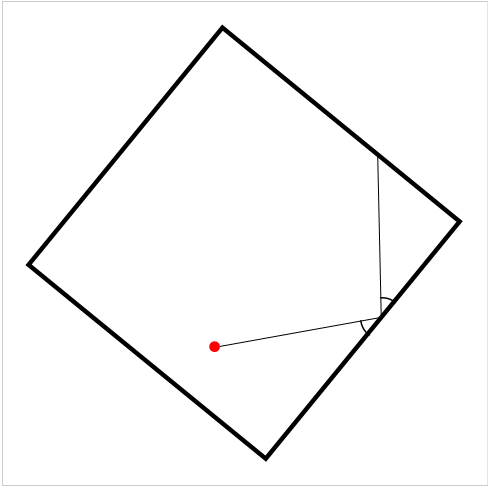
\includegraphics[width = 0.7\textwidth]{CongruentAngles}
    \caption{Square Billiard where angle of incidence equals the angle of reflection}
  \end{figure}
\end{frame}



\begin{frame}{Birkhoff Billiard}
    \begin{block}{Billiard Map}
        \begin{align*}
             f: [0, 2\pi) \times (0,\pi) &\rightarrow [0, 2\pi) \times (0,\pi) \\
             (\theta_n,\alpha_n) &\mapsto (\theta_{n+1},\alpha_{n+1})
        \end{align*}
    \end{block}
\end{frame}

\begin{frame}{Birkhoff Billiard}
  \begin{block}{What Billiard Shapes are allowed?}
  \begin{itemize}
  \item {
    Convex
  } \pause{}
  \item {
    Smooth
  }
  \end{itemize}
  \end{block}
\end{frame}

\begin{frame}{Discs}
  \begin{figure}
    \centering
    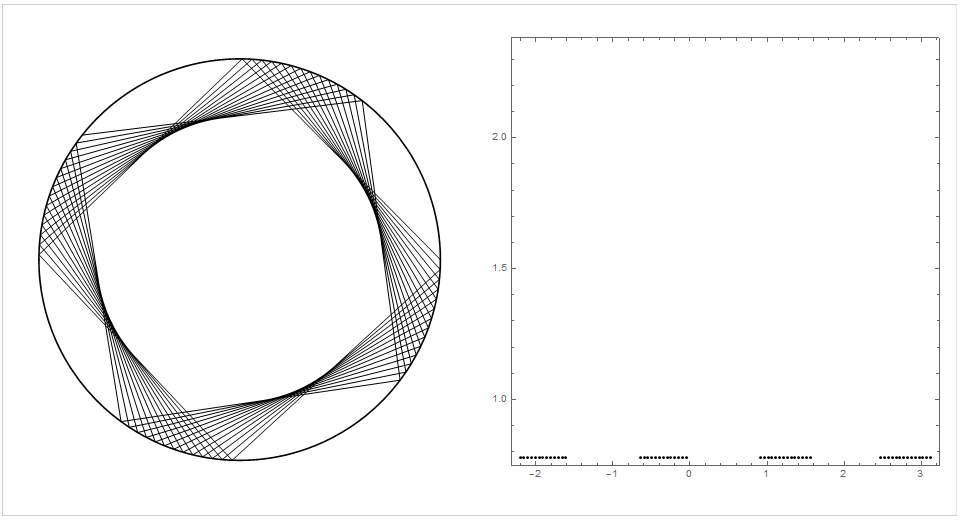
\includegraphics[width = 0.9\textwidth]{CirclePhaseSpace}
    \caption{Disc Billiard with Phase Space Diagram}
  \end{figure}
\end{frame}

\begin{frame}{Ellipse}
\begin{definition}
A curve $\Gamma \subset \Omega$ is called a \alert{caustic} of a billiard $ \Omega$ if any billiard orbit having one segment tangent to $\Gamma$ has all its sements tangent to $\Gamma$. 
\end{definition}
\end{frame}

\begin{frame}{Ellipse}
  \begin{figure}
    \centering
    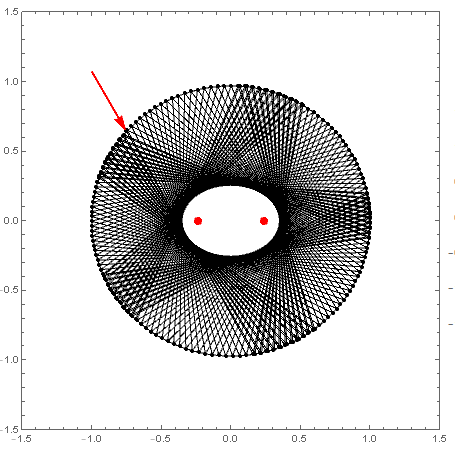
\includegraphics[width = 0.7\textwidth]{ConfocalEllipse}
    \caption{Elliptical Billiard with caustic confocal ellipse with foci shown in red}
  \end{figure}
\end{frame}

\begin{frame}{Ellipse}
  \begin{figure}
    \centering
    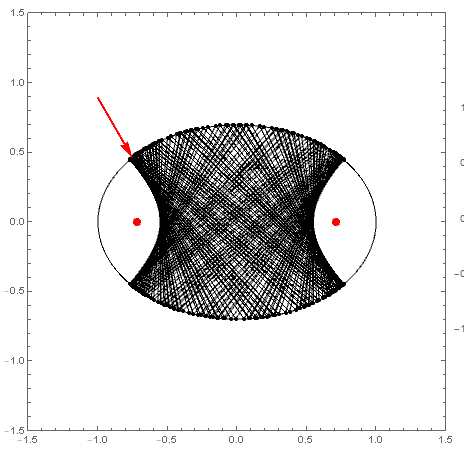
\includegraphics[width = 0.7\textwidth]{ConfocalHyperbola}
    \caption{Elliptical Billiard with caustic confocal hyperbola with foci shown in red}
  \end{figure}
\end{frame}

\begin{frame}{Ellipse}
  \begin{itemize}
  \item
    A billiard trajectory inside $\Omega$ stays tangent (caustic) to a fixed confocal ellipse or fixed confocal hyperbola.
  \end{itemize}
\end{frame}

\begin{frame}{Ellipse}
  \begin{figure}
    \centering
    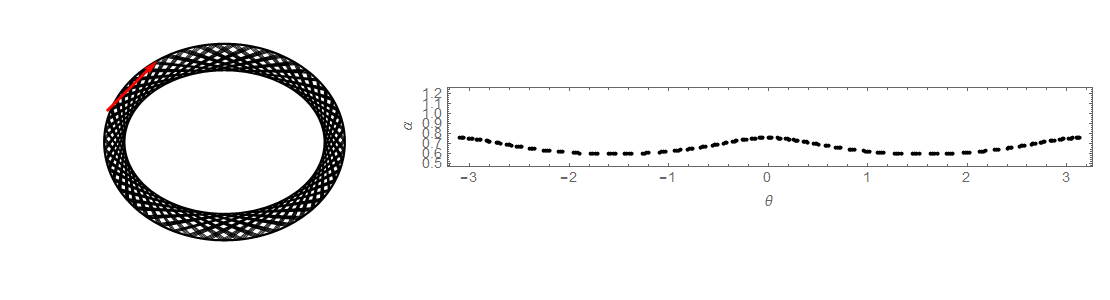
\includegraphics[width = 0.9\textwidth]{EllipsePhaseSpace}
    \caption{Elliptical Billiard with Phase Space Diagram $a = 1, b = 1.5$}
  \end{figure}
\end{frame}

\begin{frame}{Ellipse}
  \begin{figure}
    \centering
    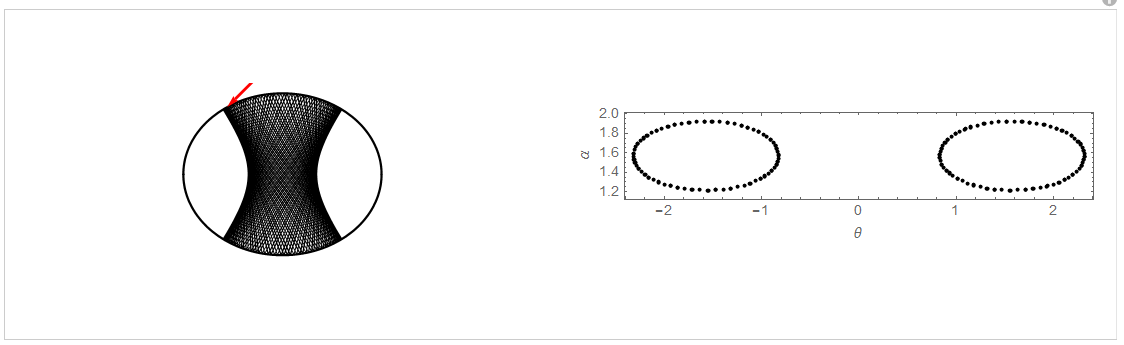
\includegraphics[width = 1\textwidth]{EllipsePhaseSpace3}
    \caption{Elliptical Billiard with Phase Space Diagram $a = 1, b = 1.5$}
  \end{figure}
\end{frame}

\begin{frame}{Ellipse}
  \begin{figure}
    \centering
    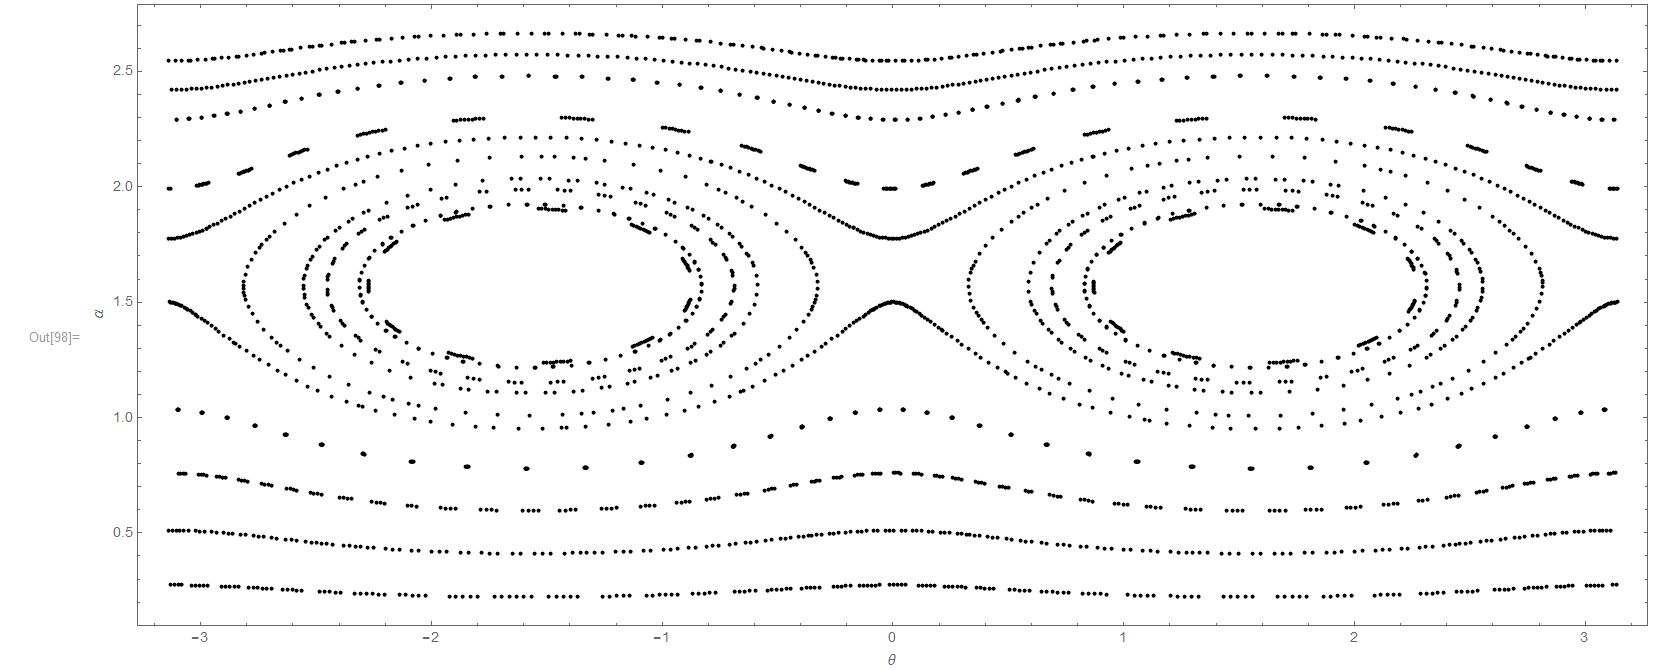
\includegraphics[width = 1\textwidth]{EllipsePhaseSpace2}
    \caption{Elliptical Billiard with Phase Space Diagram $a = 1, b = 1.5$}
  \end{figure}
\end{frame}

\begin{frame}{Ellipse}
  \begin{itemize}
  \item
    An f-invariant curve $\gamma$ in the phase space correspond to a caustic $\Gamma$. 
  \end{itemize}
\end{frame}

\begin{frame}{Near Elliptical Billiards}
Consider billiards bounded by the curves of the form 
\[
    a x^2 + b y^2 + \varepsilon x^4 = 1
\]
\end{frame}

\begin{frame}{Near Elliptical Billiards}
  \begin{figure}
    \centering
    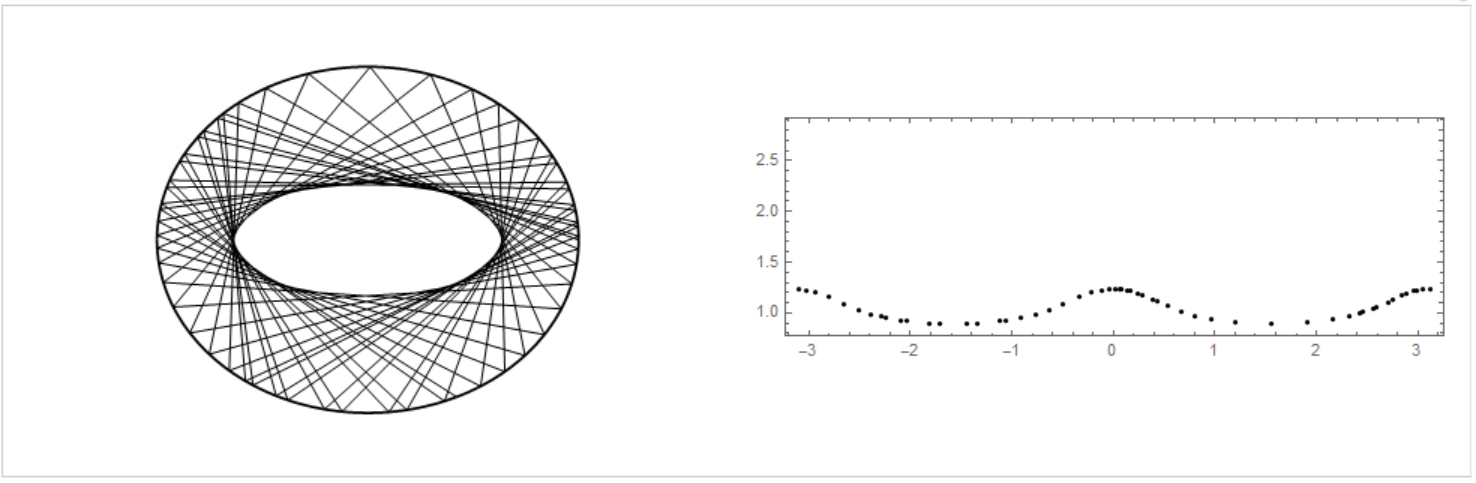
\includegraphics[width = 0.9\textwidth]{NearellipsePhaseSpace2}
    \caption{Near elliptical Billiard $a=1, b=1.5, \varepsilon = .01$ with Phase Space Diagram}
  \end{figure}
\end{frame}

\begin{frame}{Near Elliptical Billiards}
  \begin{figure}
    \centering
    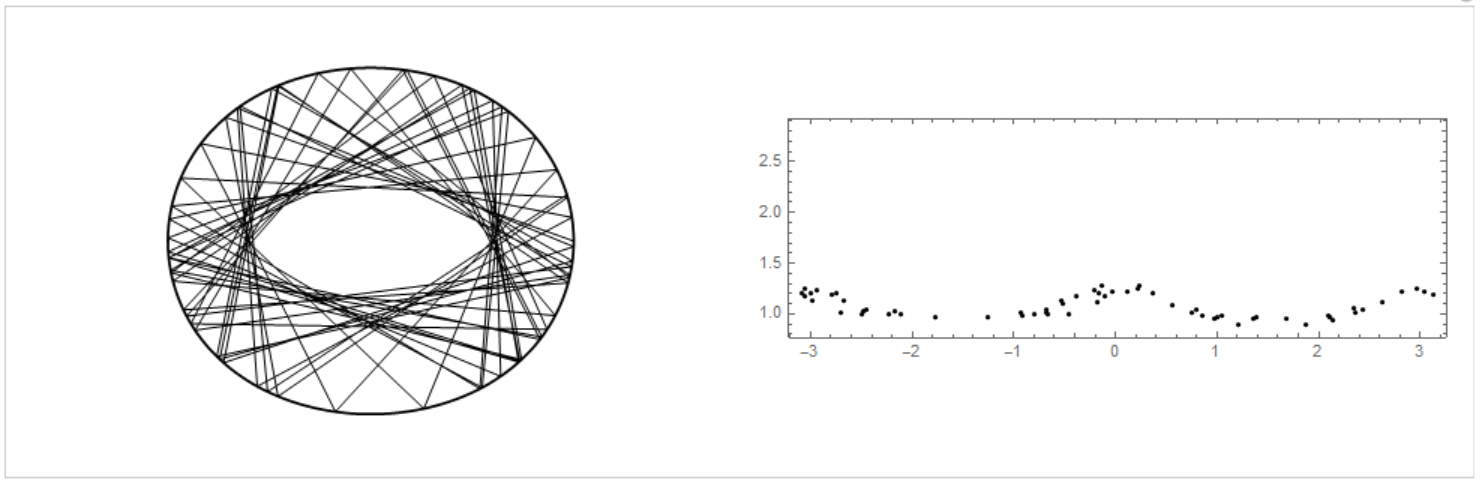
\includegraphics[width = 0.9\textwidth]{NearellipsePhaseSpace3}
    \caption{Near elliptical Billiard $a=1, b=1.5, \varepsilon = .1$ with Phase Space Diagram}
  \end{figure}
\end{frame}


\begin{frame}{Near Elliptical Billiards}
  \begin{figure}
    \centering
    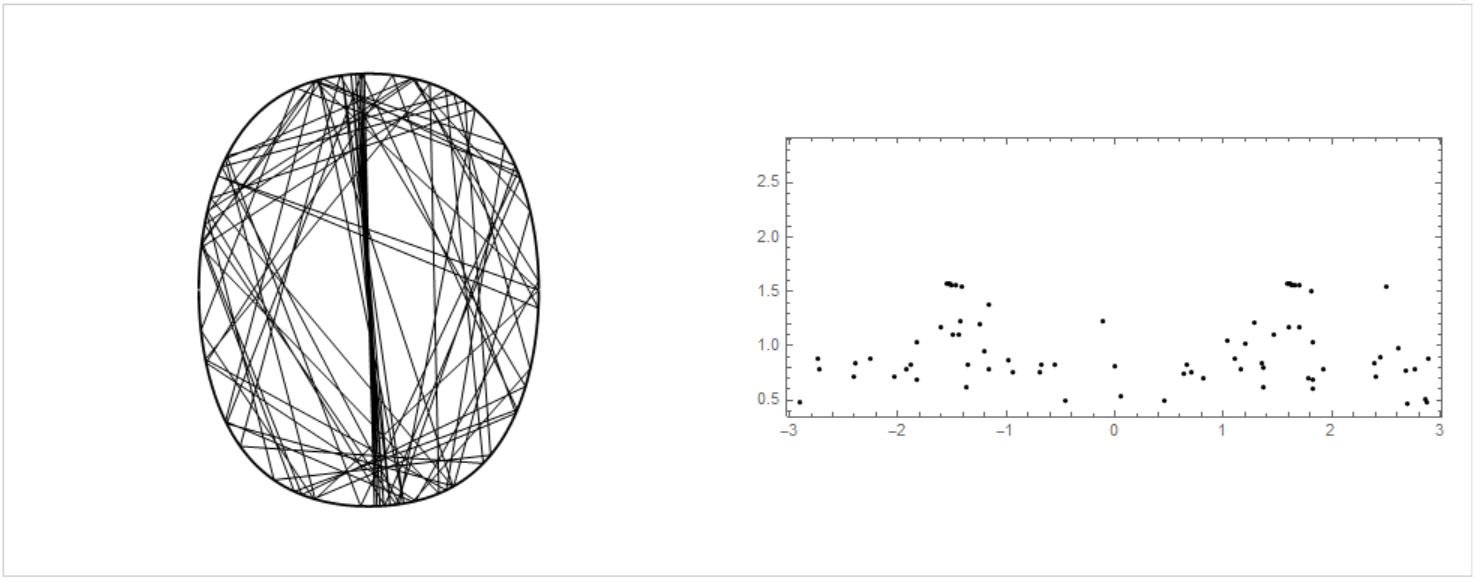
\includegraphics[width = 0.9\textwidth]{NearellipsePhaseSpace}
    \caption{Near elliptical Billiard $a=b=\varepsilon = 1$ with Phase Space Diagram}
  \end{figure}
\end{frame}

\begin{frame}{Near Elliptical Billiards}
\begin{definition}
A billiard is said to be \alert{integrable} if the union of all smooth, convex caustics, has nonempty interior.
\end{definition}
\begin{definition}
A billiard is said to be \alert{integrable} if there exists a (smooth) foliation of the whole phase space consisting of invariant
curves of the billiard map.
\end{definition}

*Note that a billiard inside an ellipse is integrable.

\end{frame}

\subsection{Birkhoff Conjecture}

% You can reveal the parts of a slide one at a time
% with the \pause command:
\begin{frame}{Birkhoff Conjecture}
  \begin{itemize}
  \item {
    \textbf{Birkhoff Conjecture} \textit{If a smooth, convex billiard in }$\Omega$ \textit{ is integrable}, \textit{then the boundary } $\partial\Omega$ \textit{ is an ellipse.}
    \pause % The slide will pause after showing the first item
  }
  \item {   
    If convex caustics completely foliate $\Omega$, then $\Omega$ is necessarily a disk. (Baily; 1993)
  }
  % You can also specify when the content should appear
  % by using <n->:
  \item<3-> {
    A small integrable perturbation of an ellipse of small eccentricity must be an ellipse. (Avila, Simoi, Kaloshin; 2016)
  }
  \item<4-> {
    A small integrable perturbation of an ellipse of arbitrary eccentricity must be an ellipse. (Kaloshin, Sorrentino; 2017)
  }
  % or you can use the \uncover command to reveal general
  % content (not just \items):
  \end{itemize}
\end{frame}

\section{Near Elliptical Billiards}

\subsection{Results}

\begin{frame}{Near Elliptical Billiards}
    Consider billiards bounded by the curves of the form 
    \begin{equation}        
        a x^2 + b y^2 + \varepsilon x^4 = 1
    \end{equation}
  The billiard mapping is definied as
    \begin{equation}
        \begin{cases} 
          F(\theta_{n+1}) = 0 = Y(\theta_{n+1}) - Y(\theta_n) - \tan(\alpha_n + \phi_n)(X(\theta_{n+1}) - X(\theta_n)) \\
          \alpha_{n+1} = \phi_{n+1} - (\alpha_n + \phi_n)
       \end{cases}
    \end{equation}
\end{frame}

\begin{frame}{Near Elliptical Billiards}
  \begin{figure}
    \centering
    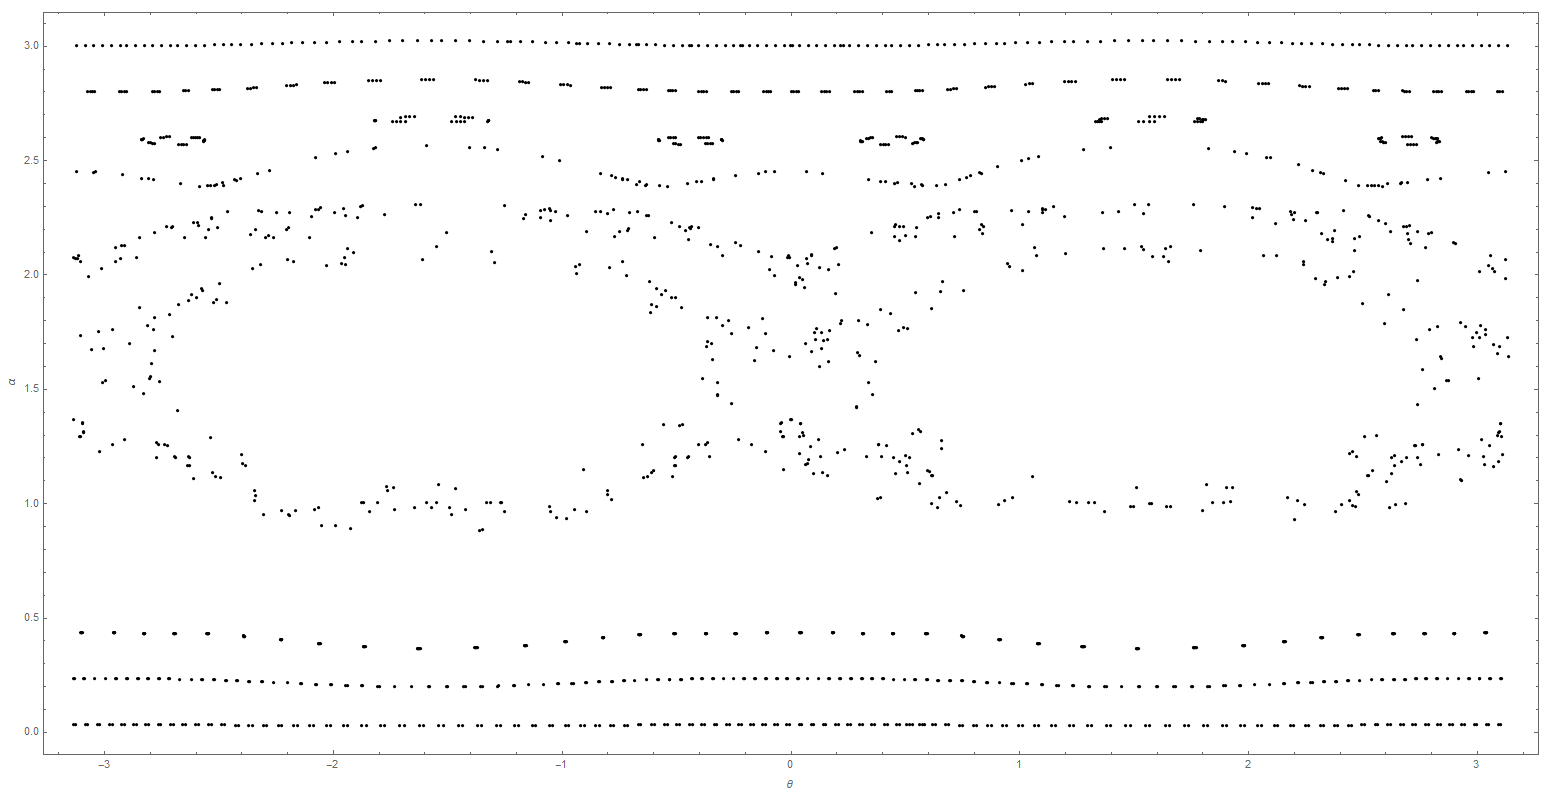
\includegraphics[width = 0.9\textwidth]{NearellipsePhaseSpace4}
    \caption{Near elliptical Billiard $a=1, b=1.5, \varepsilon = .1$ with Phase Space Diagram}
  \end{figure}
\end{frame}

\begin{frame}{Near Elliptical Billiards}
  \begin{figure}
    \centering
    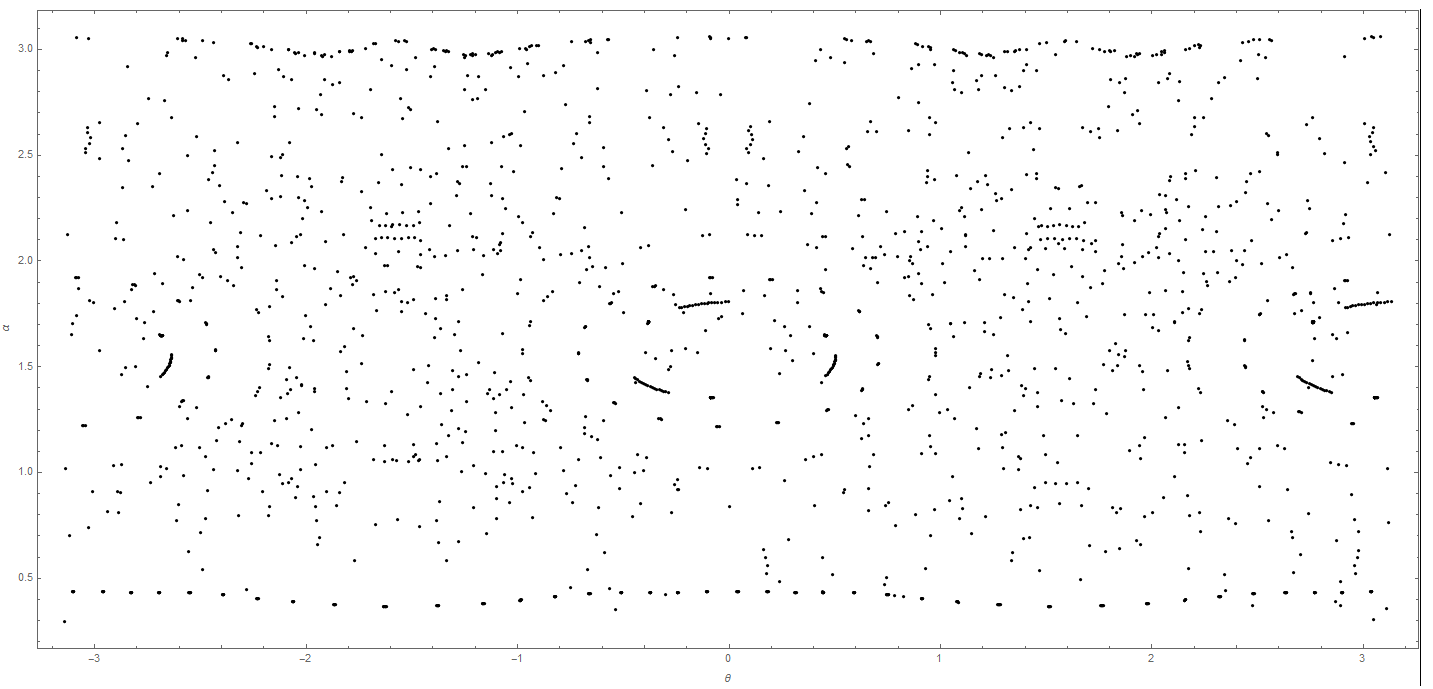
\includegraphics[width = 0.9\textwidth]{NearellipsePhaseSpace5}
    \caption{Near elliptical Billiard $a=1, b=1.5, \varepsilon = 10$ with Phase Space Diagram}
  \end{figure}
\end{frame}

\begin{frame}
  \begin{figure}
    \centering
    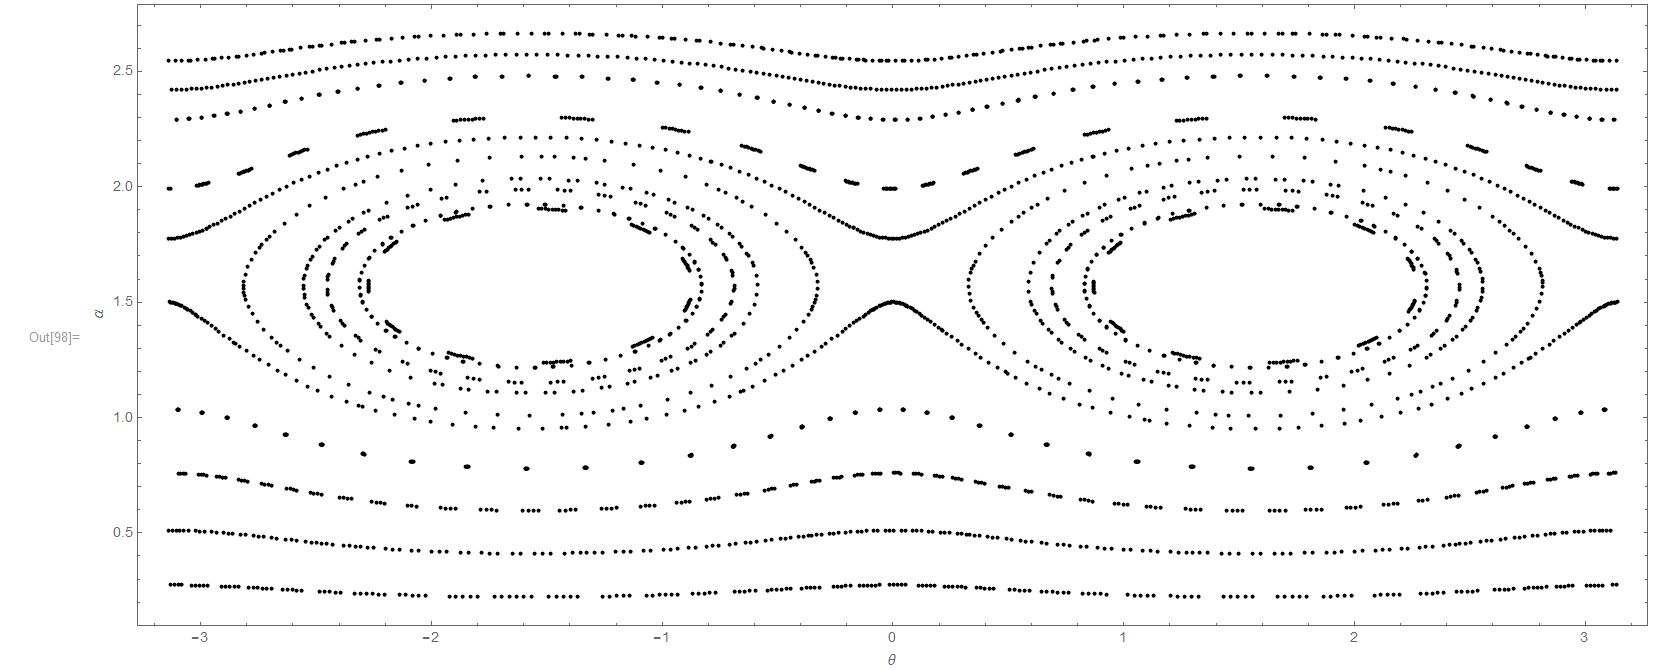
\includegraphics[width = 1\textwidth]{EllipsePhaseSpace2}
    \caption{Elliptical Billiard with Phase Space Diagram $a = 1, b = 1.5, \varepsilon = 0$}
  \end{figure}
\end{frame}

\begin{frame}{Near Elliptical Billiards}
    \begin{theorem}Mather,1982\\
     If the curvature of $d\Omega$ vanishes at some point, there exists no caustic of $\Omega$ and hence is non-integrable.
    \end{theorem}
\end{frame}

% Placing a * after \section means it will not show in the
% outline or table of contents.
\section*{Summary}

\begin{frame}{Summary}
  \begin{itemize}
  \item
    Relationship between caustics, invariant curves, and integrability.
  \item
    For $\varepsilon$ significantly large, all of the invariant curves are destroyed.
  \end{itemize}
  
  \begin{itemize}
  \item
    Outlook
    \begin{itemize}
    \item
      Sensitive dependence on initial conditions \alert{Lyapunov Exponents}
    \end{itemize}
  \end{itemize}
\end{frame}



% All of the following is optional and typically not needed. 
% \appendix
% \section<presentation>*{\appendixname}
% \subsection<presentation>*{For Further Reading}

% \begin{frame}[allowframebreaks]
%   \frametitle<presentation>{For Further Reading}
    
%   \begin{thebibliography}{10}
    
%   \beamertemplatebookbibitems
%   % Start with overview books.

%   \bibitem{Author1990}
%     A.~Author.
%     \newblock {\em Handbook of Everything}.
%     \newblock Some Press, 1990.
 
    
%   \beamertemplatearticlebibitems
%   % Followed by interesting articles. Keep the list short. 

%   \bibitem{Someone2000}
%     S.~Someone.
%     \newblock On this and that.
%     \newblock {\em Journal of This and That}, 2(1):50--100,
%     2000.
%   \end{thebibliography}
% \end{frame}

\end{document}


